\begin{figure}[ht]
\centering
%% Dummy gadget
\begin{minipage}[t]{0.3\textwidth}
    \centering
    \begin{tikzpicture}[
        nd/.style={circle, fill, inner sep=1.5pt},
        elabel/.style={midway, right, font=\small},
        clabel/.style={midway, left, font=\scriptsize},
        prec/.style={->, dashed}
    ]
        \node[nd] (v0) at (0,0) {};
        \node[nd] (v1) at (0,-1) {};
        \node[nd] (v2) at (0,-2) {};
        \node[nd] (v3) at (0,-3) {};
        \node[nd] (v4) at (0,-4) {};

        \draw (v0) -- node[elabel] {$e_1$} node[clabel] {$\brc{1}$} (v1);
        \draw (v1) -- node[elabel] {$e_2$} node[clabel] {$\brc{2}$} (v2);
        \draw (v2) -- node[elabel] {$e_3$} node[clabel] {$\brc{3}$} (v3);
        \draw (v3) -- node[elabel] {$e_4$} node[clabel] {$\brc{4}$} (v4);

        % Precedence arrows — rounded bends so they don't look like one line
        \draw[prec] ($(v0)!0.5!(v1) + (0.4,0)$) to[out=-20, in=20] ($(v1)!0.5!(v2) + (0.4,0)$);
        \draw[prec] ($(v1)!0.5!(v2) + (0.4,0)$) to[out=-20, in=20] ($(v2)!0.5!(v3) + (0.4,0)$);
        \draw[prec] ($(v2)!0.5!(v3) + (0.4,0)$) to[out=-20, in=20] ($(v3)!0.5!(v4) + (0.4,0)$);
    \end{tikzpicture}
    \subcaption{Dummy gadget}
    \label{fig:dummy-gadget}
\end{minipage}
\hfill
%% Variable gadget
\begin{minipage}[t]{0.3\textwidth}
    \centering
    \begin{tikzpicture}[
        nd/.style={circle, fill, inner sep=1.5pt},
        elabel/.style={midway, font=\small},
        clabel/.style={midway, font=\scriptsize},
        prec/.style={->, dashed}
    ]
        % Main path (two edges)
        \node[nd] (a0) at (0,0) {};
        \node[nd] (a1) at (0,-1.2) {};
        \node[nd] (a2) at (0,-2.4) {};

        \draw (a0) -- node[elabel, left] {$e_{x_i}$} node[clabel, right] {$\brc{1,2}$} (a1);
        \draw (a1) -- node[elabel, left] {$e_{\bar{x}_i}$} node[clabel, right] {$\brc{1,2}$} (a2);

        % Single-edge paths — both to the right, with more vertical separation
        \node[nd] (b0) at (2.2, 0.6) {};
        \node[nd] (b1) at (2.2,-0.4) {};
        \draw (b0) -- node[elabel, right] {$e_{x_i}'$} node[clabel, left, pos=0.3] {$\brc{2,3}$} (b1);

        \node[nd] (c0) at (2.2,-2.0) {};
        \node[nd] (c1) at (2.2,-3.0) {};
        \draw (c0) -- node[elabel, right] {$e_{\bar{x}_i}'$} node[clabel, left, pos=0.7] {$\brc{2,3}$} (c1);

        % Precedence arrows — upper: start above midpoint, end below midpoint; lower: opposite
        \draw[prec] ($(a0)!0.3!(a1)+(0.12,0)$) to[out=15, in=165] ($(b0)!0.7!(b1)+(-0.12,0)$);
        \draw[prec] ($(a1)!0.7!(a2)+(0.12,0)$) to[out=-15, in=-165] ($(c0)!0.3!(c1)+(-0.12,0)$);
    \end{tikzpicture}
    \subcaption{Variable gadget}
    \label{fig:variable-gadget}
\end{minipage}
\hfill
%% Clause gadget
\begin{minipage}[t]{0.3\textwidth}
    \centering
    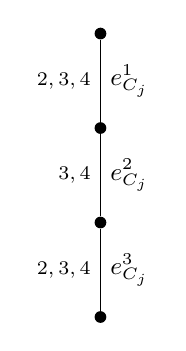
\begin{tikzpicture}[
        nd/.style={circle, fill, inner sep=1.5pt},
        elabel/.style={midway, right, font=\small},
        clabel/.style={midway, left, font=\scriptsize}
    ]
        \node[nd] (v0) at (0,0) {};
        \node[nd] (v1) at (0,-1.2) {};
        \node[nd] (v2) at (0,-2.4) {};
        \node[nd] (v3) at (0,-3.6) {};

        \draw (v0) -- node[elabel] {$e_{C_j}^1$} node[clabel] {$\brc{2,3,4}$} (v1);
        \draw (v1) -- node[elabel] {$e_{C_j}^2$} node[clabel] {$\brc{3,4}$} (v2);
        \draw (v2) -- node[elabel] {$e_{C_j}^3$} node[clabel] {$\brc{2,3,4}$} (v3);
    \end{tikzpicture}
    \subcaption{Clause gadget}
    \label{fig:clause-gadget}
\end{minipage}
\caption{Gadgets used in the reduction from 3-SAT. Edge labels are shown on the right and the sets of available colors on the left. Dashed arrows indicate precedence constraints.}
\label{fig:gadgets}
\end{figure}
